\chapter{The 4+ Windows}%
\label{cha:the_4_windows}

\section{Program Window}%
\label{sec:program_window}

The main window is called the Program window and contains the timeline as well as the entry point for all menu driven operations.  
It is often just called the “timeline”.  
The timeline consists of a vertical stack of tracks with a horizontal representation of time. 
This defines the output of rendering operations and what is saved when you save files. 
To the left of the timeline is the patchbay which contains options affecting each track.  
The patchbay is described in detail in the Editing section.

The \emph{Window} pulldown on this main window contains options that affect the 4 main windows. 
\emph{Default} positions repositions all the windows to a 4 screen editing configuration.
On dual headed displays,
the Default positions operation fills only one monitor with windows.

\subsection{Video and Audio Tracks and Navigation}%
\label{sub:video_and_audio_tracks_and_navigation}

The program window (figure~\ref{fig:pathbay})   contains many features for navigation and displays the timeline as it is structured in memory: tracks stacked vertically and extending across time horizontally. 
The horizontal scroll bar allows you to scan across time. 
The vertical scroll bar allows you to scan across tracks.

\begin{figure}[htpb]
    \centering
    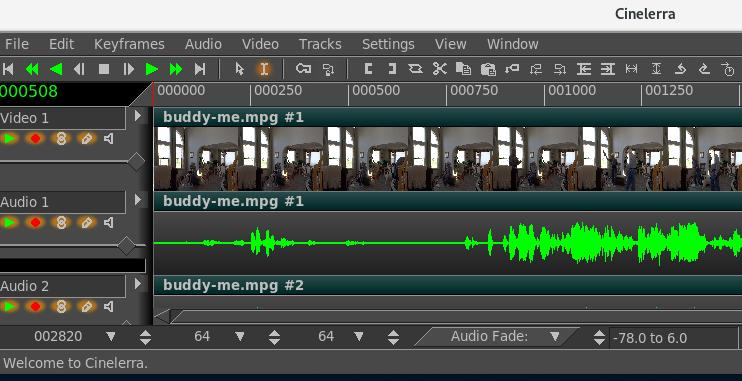
\includegraphics[width=0.8\linewidth]{images/pathbay.png}
    \caption{Patchbay  | Timeline with pulldowns \& navigation icons, Video/Audio tracks \& bottom Zoom}
    \label{fig:pathbay}
\end{figure}


Video tracks represent the duration of your videos and clips, just as if you placed real photographic film stock end-to-end on a table. 
The individual images you see on the track are samples of what is located at that particular instant on the timeline.

Audio tracks represent your sound media as an audio waveform. 
Following the film analogy, it would be as if you "viewed" magnetic tape horizontally on your table. 
You can adjust the horizontal and vertical magnification of the tracks and the magnification of the audio "waveform" display using the zoom panel controls. 
Every track on the timeline has a set of attributes on the left, called the patch- bay. 
It is used to control some of the behavior of the tracks.

Track Navigation involves both selecting a specific audio or video track and moving to a certain time in the track. 
The vertical scroll bar allows you to scan across tracks. 
For vertical scrolling you can also use the mouse wheel. 
The horizontal scroll bar allows you to scan across time. For horizontal scrolling you can use the mouse wheel with the Ctrl key.  

In addition to the graphical tools, you can use the keyboard to navigate.  
There is a shortcuts document for keyboard navigation; it includes, for example, shortcuts like use the Home and End keys to instantly go to the beginning or end of the timeline.  
Or in the default cut and paste mode, hold down Shift while pressing Home or End in order to select the region of the timeline between the insertion point and the key pressed.

\subsection{Zoom Panel}%
\label{sub:zoom_panel}

Below the timeline, you will find the zoom panel. 
The zoom panel contains values for sample zoom (duration visible on the timeline), amplitude (audio waveform scale), track zoom (height of tracks in the timeline), and curve zoom (automation range). 
In addition to the scrollbars, these zooms are the main tools for positioning the timeline.  
Also on the zoom panel is selection change and alpha slider.

\begin{figure}[htpb]
    \centering
    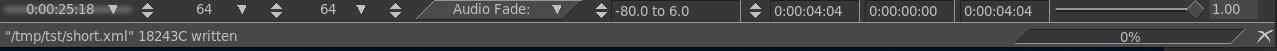
\includegraphics[width=0.99\linewidth]{images/zoompanel.png}
    \caption{Zoom panel on the bottom of the main program window}
    \label{fig:zoompanel}
\end{figure}

Changing the \emph{sample zoom} causes the unit of time displayed in the timeline to change size. 
It allows you to view your media all the way from individual frames to the entire length of your project. 
The higher the setting, the more frames you can see per screen. 
The sample zoom value is not an absolute reference for the unit of time since it refers to the duration visible on the timeline and thus changes also as you modify the length of the program window horizontally.
Use the Up and Down arrows to change the sample zoom by a power of two. 
Or if your mouse has a wheel, mouse over the tumblers and use the wheel to zoom in and out.


The \emph{amplitude} only affects audio which determines how large the waveform appears. Ctrl-up and Ctrl-down cause the amplitude zoom to change.

The \emph{track zoom} affects all tracks. 
It determines the height of each track. 
If you change the track zoom, the amplitude zoom compensates so that the audio waveforms look proportional. 
Ctrl-pgup and Ctrl-pgdown cause the track zoom to change.

The \emph{curve zoom} affects the curves in all the tracks of the same type. 
It determines the value range for curves. 
First select the automation type (audio fade, video fade, zoom, X,Y) then use the left tumblers for the minimum value and the right tumblers for the maximum value or manually enter the values in the text box. 
Normally you will use -40.0 to 6.0 for audio fade and 0.0 to 100.0 for video fade. 
The tumblers change curve amplitude, but the only way to curve offset is to use the fit curves button.

The \emph{selection start time}, \emph{selection length}, and \emph{selection end time} display the current selected timeline values.  
The \emph{alpha slider} allows for varying the alpha value when using colors on the tracks as set in your appearance preferences for Autocolor assets.  
It has no function without that flag set.

\subsection{Track Popup Menu}%
\label{sub:track_popup_menu}

Each Track has a popup menu. 
To activate the track popup menu, Right mouse click on the track. 
The popup menu affects the track whether the track is armed on the patchbay or not. 
The Track Menu contains a number of options:

\begin{description}
    \item[Attach Effect] opens a dialog box of effects applicable to the type of track of audio or video.
    \item[Move up] moves the selected track one step up in the stack.
    \item[Move down]  moves the selected track one step down in the stack.
    \item[Delete track]  removes the track from the timeline.
    \item[Add Track]  adds a track of the same media type, audio or video, as the one selected above that track.
    \item[Find in Resources]  that media file will be highlighted in the media folder in the Resources window.
    \item[Show edit]  will point out the exact start and stop points along with the length of the current edit on
        that track as well as the media name.
    \item[User title]  is used to change the title name.  This is really handy for files that have very long and
        similar names that would get cut off during edits.  You can use short names to better differentiate the
        media. If you select multiple, all those clips will have title name changed.
    \item[Bar color]  allows the user to select a specific color for the title bar.  This helps ease of locating.
    \item[Resize Track]  resizes the track.
    \item[Match Output Size]  resizes the track to match the current output size.
\end{description}


\subsection{Insertion Point}%
\label{sub:insertion_point}

The insertion point (figure~\ref{fig:insertion-points}) is the flashing hairline mark that vertically spans the timeline in the program window. 
Analogous to the cursor on your word processor, the insertion point marks the place on the timeline where the next activity will begin. 
It is the point where a paste operation takes place. 
When rendering, it defines the beginning of the region of the timeline to be rendered. It is also the starting point of all playback operations.
                           
Normally, the insertion point is moved by clicking inside the main timebar. 
Any region of the timebar not obscured by labels and in or out points is a hotspot for repositioning the insertion point. 
In cut and paste editing mode only, the insertion point can be moved also by clicking in the timeline itself. 
When moving the insertion point the position is either aligned to frames or aligned to samples. 
When editing video, you will want to align to frames. When editing audio you will want to align to samples. Select your preference by using Settings->Align cursor on frames.

\begin{figure}[htpb]
    \centering
    %\includegraphics[width=0.8\linewidth]{name.ext}
    \begin{tikzpicture}[scale=1, transform shape]
        \node (img1) [yshift=0cm, xshift=0cm, rotate=0] {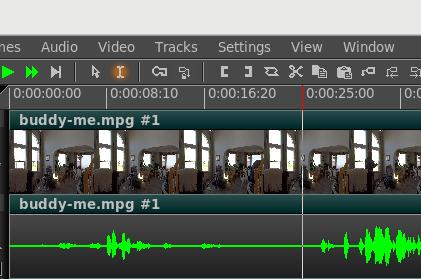
\includegraphics[width=0.6\linewidth]{images/insertion-point.png}};
        \node [yshift=-13mm, xshift=-1cm,anchor=east] at (img1.north west) (Pulldowns) {Pulldowns};
        \node [yshift=-20mm, xshift=-1cm,anchor=east] at (img1.north west) (Transport) {Transport \& Buttons Bar};
        \node [yshift=-27mm, xshift=-1cm,anchor=east] at (img1.north west) (Timebar) {Timebar};
        \node [yshift=-33mm, xshift=-1cm,anchor=east] at (img1.north west) (Title) {Media Title };
        \node [yshift=-43mm, xshift=-1cm,anchor=east] at (img1.north west) (Video) {Video Track};
        \node [yshift=-63mm, xshift=-1cm,anchor=east] at (img1.north west) (Audio) {Audio Track};
        \draw [->, line width=1mm] (Pulldowns) edge  ([yshift=-13mm] img1.north west);
        \draw [->, line width=1mm] (Transport) edge  ([yshift=-20mm] img1.north west);
        \draw [->, line width=1mm] (Timebar) edge    ([yshift=-27mm] img1.north west);
        \draw [->, line width=1mm] (Title) edge      ([yshift=-33mm] img1.north west);
        \draw [->, line width=1mm] (Video) edge      ([yshift=-43mm] img1.north west);
        \draw [->, line width=1mm] (Audio) edge      ([yshift=-63mm] img1.north west);
        \end{tikzpicture}
    
    \caption{Insertion point is at 0:00:25:10 in Hr:Mn:Sec:Frames}
    \label{fig:insertion-points}
\end{figure}


\subsection{Editing Modes}%
\label{sub:editing_modes}

There are 2 different editing methods of operation that affect the insertion point and the editing on the timeline.  
There is:  \emph{drag and drop mode} and \emph{cut and paste mode}. 
The editing mode is determined by selecting the arrow or the I-beam in the Transport and Buttons bar. 

If the arrow is highlighted, it enables \emph{drag and drop mode}.  
In drag and drop mode, clicking in the timeline does not reposition the insertion point.  
Double-clicking in the timeline selects the entire edit the mouse pointer is over.  
Dragging in the timeline repositions the edit the mouse pointer is over. 
This is useful for reordering audio playlists, sorting movie scenes, or moving effects around. 
To cut and paste in drag and drop mode you need to set in/out points to define an affected region. 

If the I-beam is highlighted it enables \emph{cut and paste mode}. 
In cut and paste mode, clicking in the timeline repositions the insertion point. 
Double-clicking in the timeline selects the entire edit the cursor is over. 
Dragging in the timeline highlights a region. 
The highlighted region becomes the region affected by cut and paste operations and the playback range during the next playback operation. 
Shift-clicking in the timeline extends the highlighted region.

When highlighting a region, the start and end points are either aligned to frames or aligned to samples. When editing video, you will want to align to frames. When editing audio you will want to align to samples. Select your preference by using settings->align cursor on frames.

\begin{figure}[htpb]
    \centering
    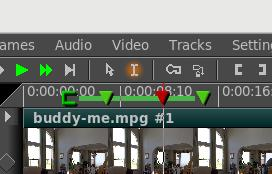
\includegraphics[width=0.4\linewidth]{images/i-beam.png}
    \caption{I-beam + in/out  +  labels}
    \label{fig:i-beam}
\end{figure}

\subsection{In/Out Points}%
\label{sub:in_out_points}

In both editing modes, you can set one In point and one Out point. 
The in/out points define the affected region. 
In drag and drop mode, they are the only way to define an affected region. 
In both cut and paste mode and drag and drop mode, the highlighted area overrides the In/Out points. 
If a highlighted area and In/Out points are set, the highlighted area is affected by editing operations and the In/Out points are ignored. 
If no region is highlighted, the In/Out points are used. 
To avoid confusion, it is better to use either highlighting or In/Out points but not both simultaneously.

To set in/out points, go to the timebar and position the insertion point somewhere. 
Select the In point button. 
Move the insertion point to a position after the In point and click the Out point button. 
Instead of using the button bar, you can use the [ or < and ] or > keys to toggle in/out points.

If you set the insertion point somewhere else while In/Out points already exist, when you click the In/Out buttons the existing points will be repositioned. 
If you click on in/out points while a region is highlighted, the insertion point will be ignored and In/Out points will be set at the beginning and at the end of the highlighted area.

If you select either the In point or the Out point, the insertion point will jump to that location. 
After selecting an In point, if you click the In point button the In point will be deleted. 
After selecting an Out point, if you click the Out point button the Out point will be deleted. 
Shift-clicking on an In/Out point highlights the region between the insertion point and that In/Out point. 
If a region is already highlighted, it extends the highlighted region up to that In/Out point.

To quickly get rid of In/Out points, without caring about where they are or if they are set or not, just double click on [ and ] buttons. 
The first click will set a new point or reposition an old one at the insertion point; the second click will delete it. This trick does not work if the In point or the Out point is already set at insertion point.

Some of the useful operations concerning the In/Out pointers are listed next.

\begin{description}
    \item[Ctrl-KeyPad\#]  if in/out set, KP 2,3,5,6 + Enter, play between In/Out point
    \item[Shift-Ctrl]  loops play between In/Out points
    \item[Click in/out] while holding the left mouse button, drags In/Out pointer elsewhere
    \item[Shift-Ctrl] with transport button, loops play between In/Out points
    \item[Ctrl-t]  clears both In/Out points
\end{description}

\subsection{Labels}%
\label{sub:labels}



